\documentclass{standalone}
\usepackage{tikz}
\usetikzlibrary{patterns, positioning}
\usepackage[sfdefault]{ClearSans} %% option 'sfdefault' activates Clear Sans as the default text font
\usepackage[T1]{fontenc}

\begin{document}
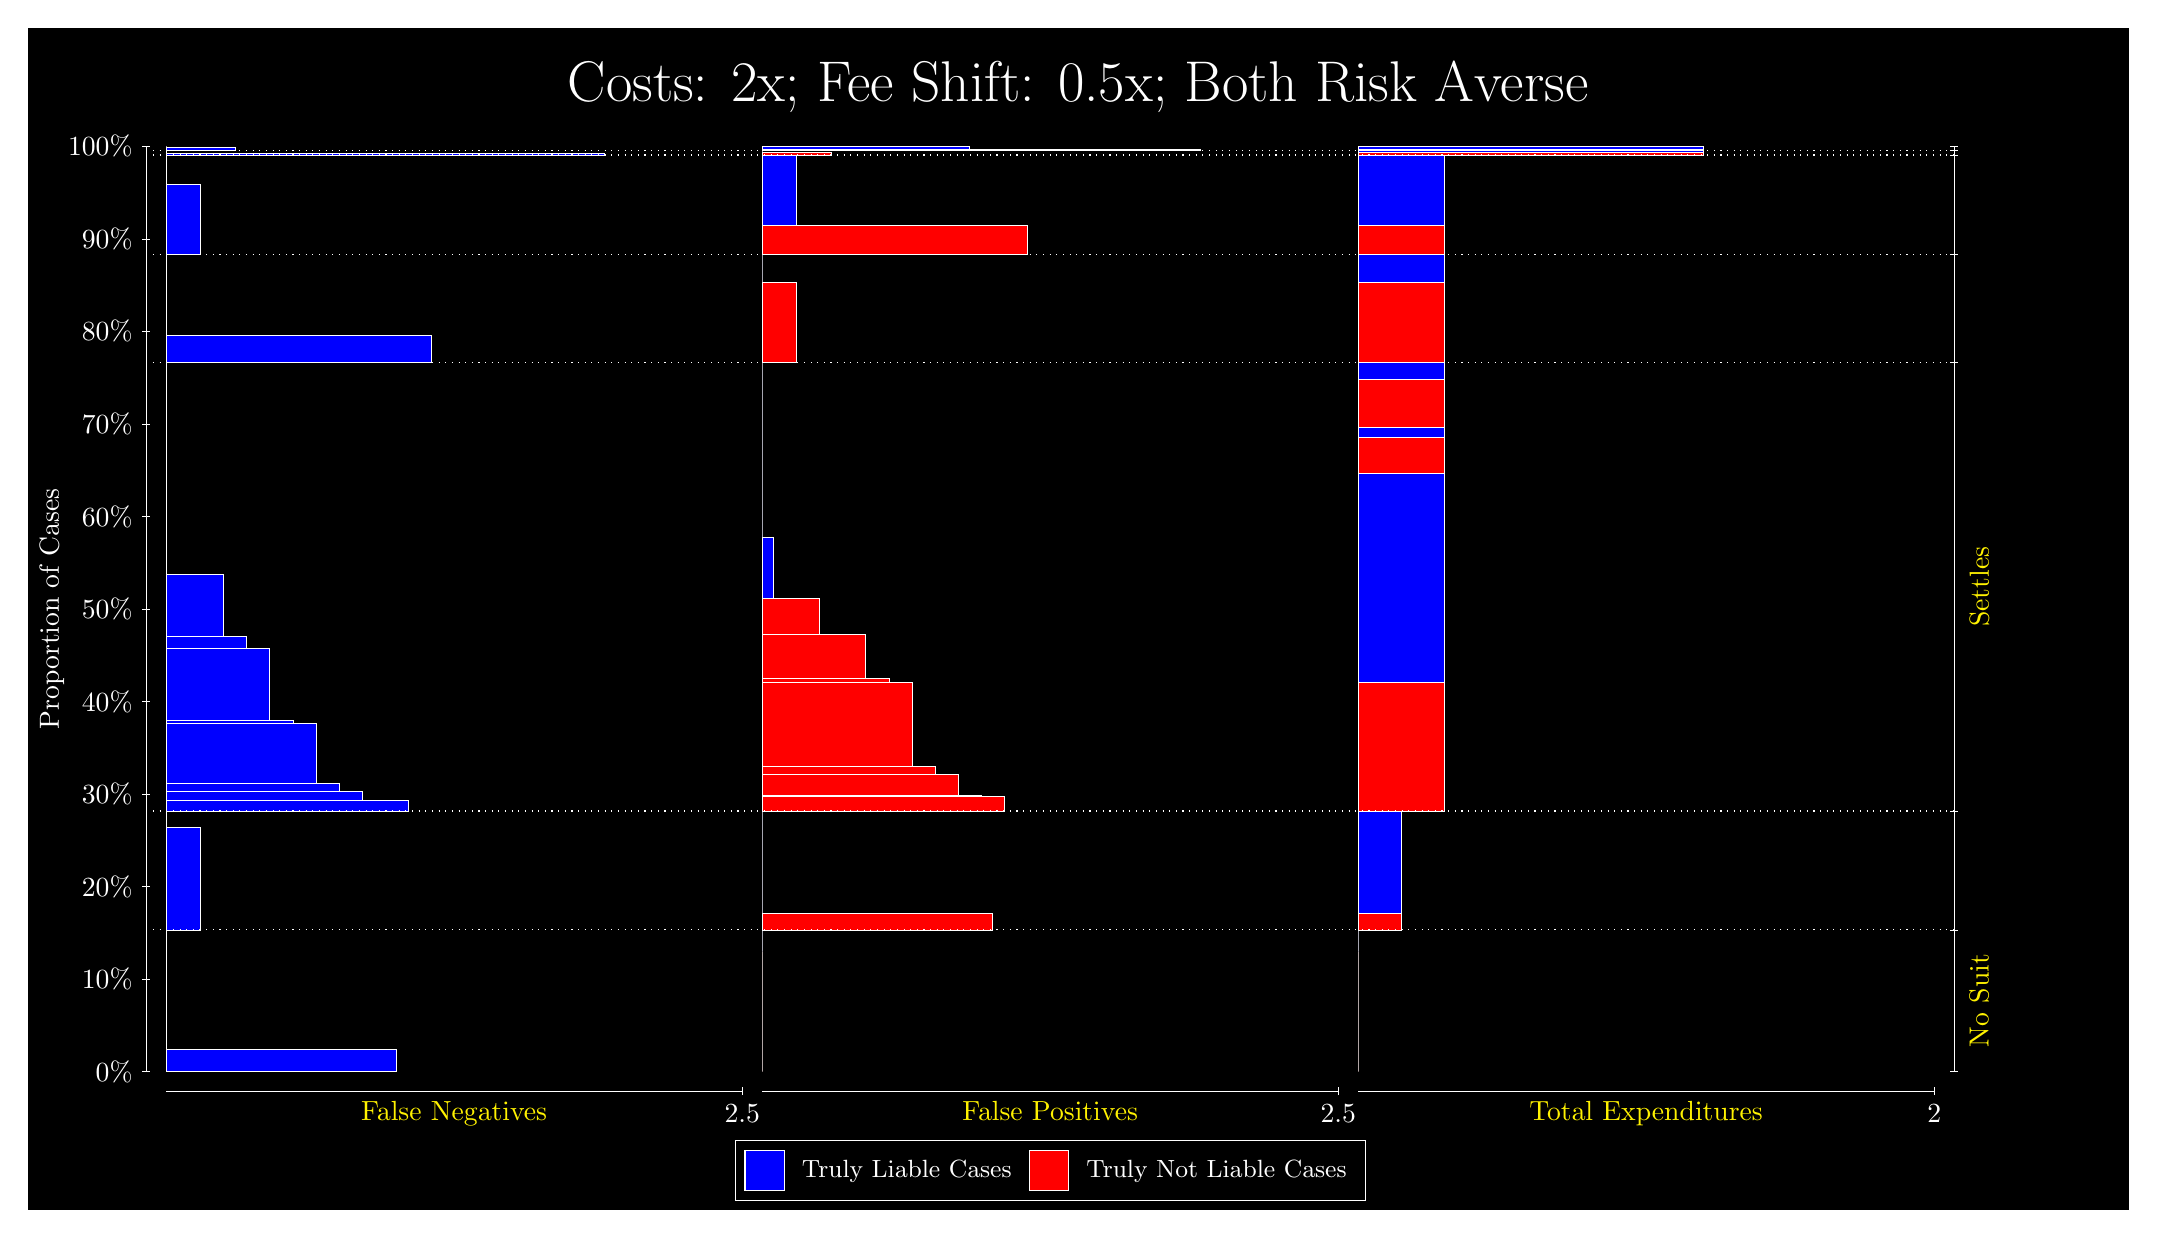
\begin{tikzpicture}
\draw[fill=black] (0,0) rectangle (26.667,15);
\draw[text=white] (0,13.5) rectangle (26.667,15) node[midway] {\huge Costs: 2x; Fee Shift: 0.5x; Both Risk Averse};
\draw[white, very thin] (1.5,1.75) -- (1.5,13.5);
\node[rotate=90, text=white, anchor=center] at (0.3, 7.625) {Proportion of Cases};
\draw[white, very thin] (1.45,1.75) -- (1.55,1.75);
\node[text=white, anchor=east] at (1.45, 1.75) {0\%};
\draw[white, very thin] (1.45,2.925) -- (1.55,2.925);
\node[text=white, anchor=east] at (1.45, 2.925) {10\%};
\draw[white, very thin] (1.45,4.1) -- (1.55,4.1);
\node[text=white, anchor=east] at (1.45, 4.1) {20\%};
\draw[white, very thin] (1.45,5.275) -- (1.55,5.275);
\node[text=white, anchor=east] at (1.45, 5.275) {30\%};
\draw[white, very thin] (1.45,6.45) -- (1.55,6.45);
\node[text=white, anchor=east] at (1.45, 6.45) {40\%};
\draw[white, very thin] (1.45,7.625) -- (1.55,7.625);
\node[text=white, anchor=east] at (1.45, 7.625) {50\%};
\draw[white, very thin] (1.45,8.8) -- (1.55,8.8);
\node[text=white, anchor=east] at (1.45, 8.8) {60\%};
\draw[white, very thin] (1.45,9.975) -- (1.55,9.975);
\node[text=white, anchor=east] at (1.45, 9.975) {70\%};
\draw[white, very thin] (1.45,11.15) -- (1.55,11.15);
\node[text=white, anchor=east] at (1.45, 11.15) {80\%};
\draw[white, very thin] (1.45,12.325) -- (1.55,12.325);
\node[text=white, anchor=east] at (1.45, 12.325) {90\%};
\draw[white, very thin] (1.45,13.5) -- (1.55,13.5);
\node[text=white, anchor=east] at (1.45, 13.5) {100\%};

\draw[white, very thin] (24.457,1.75) -- (24.457,13.5);
\draw[white, very thin] (24.407,1.75) -- (24.507,1.75);
\node[anchor=west] at (24.407, 1.75) {};
\draw[white, very thin] (24.407,3.5497) -- (24.507,3.5497);
\node[anchor=west] at (24.407, 3.5497) {};
\draw[white, very thin] (24.407,5.0587) -- (24.507,5.0587);
\node[anchor=west] at (24.407, 5.0587) {};
\draw[white, very thin] (24.407,10.757) -- (24.507,10.757);
\node[anchor=west] at (24.407, 10.757) {};
\draw[white, very thin] (24.407,12.124) -- (24.507,12.124);
\node[anchor=west] at (24.407, 12.124) {};
\draw[white, very thin] (24.407,13.39) -- (24.507,13.39);
\node[anchor=west] at (24.407, 13.39) {};
\draw[white, very thin] (24.407,13.446) -- (24.507,13.446);
\node[anchor=west] at (24.407, 13.446) {};
\draw[white, very thin] (24.407,13.5) -- (24.507,13.5);
\node[anchor=west] at (24.407, 13.5) {};

\draw[white, very thin, fill=blue] (1.75,1.75) rectangle (4.6775,2.0281);
\draw[white, very thin, fill=red] (1.75,2.0281) rectangle (1.75,3.5497);
\draw[white, very thin, fill=blue] (1.75,3.5497) rectangle (2.1891,4.8478);
\draw[white, very thin, fill=red] (1.75,4.8478) rectangle (1.75,5.0587);
\draw[white, very thin, fill=blue] (1.75,5.0587) rectangle (4.8239,5.1901);
\draw[white, very thin, fill=blue] (1.75,5.1901) rectangle (4.2384,5.3048);
\draw[white, very thin, fill=blue] (1.75,5.3048) rectangle (3.9457,5.4078);
\draw[white, very thin, fill=blue] (1.75,5.4078) rectangle (3.6529,6.178);
\draw[white, very thin, fill=blue] (1.75,6.178) rectangle (3.3602,6.2125);
\draw[white, very thin, fill=blue] (1.75,6.2125) rectangle (3.0674,7.1191);
\draw[white, very thin, fill=blue] (1.75,7.1191) rectangle (2.7746,7.2822);
\draw[white, very thin, fill=blue] (1.75,7.2822) rectangle (2.4819,8.0619);
\draw[white, very thin, fill=red] (1.75,8.0619) rectangle (1.75,10.757);
\draw[white, very thin, fill=blue] (1.75,10.757) rectangle (5.1167,11.106);
\draw[white, very thin, fill=red] (1.75,11.106) rectangle (1.75,12.124);
\draw[white, very thin, fill=blue] (1.75,12.124) rectangle (2.1891,13.017);
\draw[white, very thin, fill=red] (1.75,13.017) rectangle (1.75,13.39);
\draw[white, very thin, fill=blue] (1.75,13.39) rectangle (7.3123,13.407);
\draw[white, very thin, fill=red] (1.75,13.407) rectangle (1.75,13.446);
\draw[white, very thin, fill=blue] (1.75,13.446) rectangle (2.6283,13.484);
\draw[white, very thin, fill=red] (1.75,13.484) rectangle (1.75,13.5);
\draw[white, very thin, fill=red] (9.3189,1.75) rectangle (9.3189,3.2717);
\draw[white, very thin, fill=blue] (9.3189,3.2717) rectangle (9.3189,3.5497);
\draw[white, very thin, fill=red] (9.3189,3.5497) rectangle (12.246,3.7607);
\draw[white, very thin, fill=blue] (9.3189,3.7607) rectangle (9.3189,5.0587);
\draw[white, very thin, fill=red] (9.3189,5.0587) rectangle (12.393,5.2406);
\draw[white, very thin, fill=red] (9.3189,5.2406) rectangle (12.1,5.2629);
\draw[white, very thin, fill=red] (9.3189,5.2629) rectangle (11.807,5.5245);
\draw[white, very thin, fill=red] (9.3189,5.5245) rectangle (11.515,5.6251);
\draw[white, very thin, fill=red] (9.3189,5.6251) rectangle (11.222,6.6932);
\draw[white, very thin, fill=red] (9.3189,6.6932) rectangle (10.929,6.7388);
\draw[white, very thin, fill=red] (9.3189,6.7388) rectangle (10.636,7.3011);
\draw[white, very thin, fill=red] (9.3189,7.3011) rectangle (10.051,7.7541);
\draw[white, very thin, fill=blue] (9.3189,7.7541) rectangle (9.4652,8.5338);
\draw[white, very thin, fill=blue] (9.3189,8.5338) rectangle (9.3189,10.757);
\draw[white, very thin, fill=red] (9.3189,10.757) rectangle (9.758,11.776);
\draw[white, very thin, fill=blue] (9.3189,11.776) rectangle (9.3189,12.124);
\draw[white, very thin, fill=red] (9.3189,12.124) rectangle (12.686,12.497);
\draw[white, very thin, fill=blue] (9.3189,12.497) rectangle (9.758,13.39);
\draw[white, very thin, fill=red] (9.3189,13.39) rectangle (10.197,13.429);
\draw[white, very thin, fill=blue] (9.3189,13.429) rectangle (9.3189,13.446);
\draw[white, very thin, fill=red] (9.3189,13.446) rectangle (14.881,13.462);
\draw[white, very thin, fill=blue] (9.3189,13.462) rectangle (11.954,13.5);
\draw[white, very thin, fill=red] (16.888,1.75) rectangle (16.888,3.2717);
\draw[white, very thin, fill=blue] (16.888,3.2717) rectangle (16.888,3.5497);
\draw[white, very thin, fill=red] (16.888,3.5497) rectangle (17.437,3.7607);
\draw[white, very thin, fill=blue] (16.888,3.7607) rectangle (17.437,5.0587);
\draw[white, very thin, fill=red] (16.888,5.0587) rectangle (17.986,6.6932);
\draw[white, very thin, fill=blue] (16.888,6.6932) rectangle (17.986,9.3474);
\draw[white, very thin, fill=red] (16.888,9.3474) rectangle (17.986,9.8003);
\draw[white, very thin, fill=blue] (16.888,9.8003) rectangle (17.986,9.9317);
\draw[white, very thin, fill=red] (16.888,9.9317) rectangle (17.986,10.54);
\draw[white, very thin, fill=blue] (16.888,10.54) rectangle (17.986,10.757);
\draw[white, very thin, fill=red] (16.888,10.757) rectangle (17.986,11.776);
\draw[white, very thin, fill=blue] (16.888,11.776) rectangle (17.986,12.124);
\draw[white, very thin, fill=red] (16.888,12.124) rectangle (17.986,12.497);
\draw[white, very thin, fill=blue] (16.888,12.497) rectangle (17.986,13.39);
\draw[white, very thin, fill=red] (16.888,13.39) rectangle (21.279,13.429);
\draw[white, very thin, fill=blue] (16.888,13.429) rectangle (21.279,13.446);
\draw[white, very thin, fill=red] (16.888,13.446) rectangle (21.279,13.462);
\draw[white, very thin, fill=blue] (16.888,13.462) rectangle (21.279,13.5);
\draw[white, dotted] (1.5,3.5497) -- (24.457,3.5497);
\draw[white, dotted] (1.5,5.0587) -- (24.457,5.0587);
\draw[white, dotted] (1.5,10.757) -- (24.457,10.757);
\draw[white, dotted] (1.5,12.124) -- (24.457,12.124);
\draw[white, dotted] (1.5,13.39) -- (24.457,13.39);
\draw[white, dotted] (1.5,13.446) -- (24.457,13.446);
\draw[white, very thin] (1.75,1.5) -- (9.0689,1.5);
\node[text=yellow, anchor=north] at (5.4094, 1.5) {False Negatives};
\draw[white, very thin] (9.0689,1.45) -- (9.0689,1.55);
\node[text=white, anchor=north] at (9.0689, 1.45) {2.5};

\draw[white, very thin] (9.3189,1.5) -- (16.638,1.5);
\node[text=yellow, anchor=north] at (12.978, 1.5) {False Positives};
\draw[white, very thin] (16.638,1.45) -- (16.638,1.55);
\node[text=white, anchor=north] at (16.638, 1.45) {2.5};

\draw[white, very thin] (16.888,1.5) -- (24.207,1.5);
\node[text=yellow, anchor=north] at (20.547, 1.5) {Total Expenditures};
\draw[white, very thin] (24.207,1.45) -- (24.207,1.55);
\node[text=white, anchor=north] at (24.207, 1.45) {2};

\node[text=yellow, centered, rotate=90] at (24.777, 2.6499) {No Suit};

\node[text=yellow, centered, rotate=90] at (24.777, 7.908) {Settles};





\draw (12.978300999999998,1.5) node[draw=none] (baseCoordinate) {};
\begin{scope}[align=center]
        \matrix[scale=0.5, draw=white, below=0.5cm of baseCoordinate, nodes={draw}, column sep=0.1cm]{
            \node[rectangle, draw, minimum width=0.5cm, minimum height=0.5cm, fill=blue] {}; &
            \node[draw=none, font=\small, text=white] (B) {Truly Liable Cases}; &
            \node[rectangle, draw, minimum width=0.5cm, minimum height=0.5cm, fill=red] {}; &
            \node[draw=none, font=\small, text=white] (B) {Truly Not Liable Cases}; \\
            };
\end{scope}

\end{tikzpicture}
\end{document}